\documentclass[10pt,a4paper,twoside]{jarticle}
%==== 科研費LaTeX =============================================
%	2015(H27)年度 DC
%============================================================
% 2008-03-08: Taku Yamanaka (JSPS Research Center for Science Systems / Osaka Univ.)
% 2009-03-03: Yoko Yanagida (Assistant)
% 2010-03-03: Taku: Imported new features introduced in 2009 fall.
% 2011-02-25: Taku: Revised for JFY2013.
% 2013-03-14: Taku: Revised for JFY2014.
%============================================================
%=======================================
% form00_header.tex
%	General header for kakenhiLaTeX,  Moved over from form00_2010_header.tex.
%	2009-09-06 Taku Yamanaka (Osaka Univ.)
%==== General Version History ======================================
% 2006-05-30 Taku Yamanaka (Physics Dept., Osaka Univ.)
% 2006-06-02 V1.0
% 2006-06-14 V1.1 Use automatic calculation for cost tables.
% 2006-06-18 V1.2 Split user's contents and the format.
% 2006-06-20 V1.3 Reorganized user and format files
% 2006-06-25 V1.4 Readjusted all the table column widths with p{...}.
%				With \KLTabR and \KLTabRNum, now the items can be right-justified
%				in the cell defined by p{...}.
% 2006-06-26 V1.5 Use \newlength and \setlength, instead of \newcommand, to define positions.
% 2006-08-19 V1.6 Remade it for 2007 JFY version.
% 2006-09-05 V1.7 Added font declarations suggested by Hoshino@Meisei Univ.
% 2006-09-06 V1.8 Introduced usePDFform flag to switch the form file format.
% 2006-09-09 V1.9 Changed p.7, to allow different heights between years. (Thanks to Ytow.)
% 2006-09-11 V2.0 Added an option to show budget summary.
% 2006-09-13 V2.1 Added an option to show the group.
% 2006-09-14 V2.1.1 Cleaned up Kenkyush Chosho.
% 2006-09-21 V2.2 Generated under a new automatic development system.

% 2007-03-24 V3.0 Switched to a method using "picture" environment.

% 2007-08-14 V3.1 Switched to kakenhi3.sty.
% 2007-09-17 V3.2 Added \KLMaxYearCount
% 2008-03-08 V3.3 Remade it for 2009 JFY version\
% 2008-09-08 V3.4 Added \KLXf ... \KLXh.
% 2011-10-20 V5.0 Use kakenhi5.sty, to utilize array package in tabular environment.
% 2012-08-14 v5.1 Moved preamble and kakenhi5 into the current directory, instead of the parent directory.
% 2012-11-10 v6.0 Switched to kakenhi6.sty.
%=======================================
%============================================================
% preamble.tex
%
% Dummy section and subsection commands.
% With these, some editors (such as TeXShop, etc.) can jump to the (sub)sections.
\newcommand{\dummy}{dummy}% 
\renewcommand{\section}[1]{\renewcommand{\dummy}{#1}}
\renewcommand{\subsection}[1]{\renewcommand{\dummy}{#1}}

% Flag for switching form file format.......
\usepackage{ifthen}
\newboolean{usePDFform}
\newboolean{BudgetSummary}

\usepackage{forms/kakenhi6}

\pagestyle{empty}

% ===== Parameters for LaTeX =========================

% ===== Font declarations  ======================================
\DeclareFontShape{JT1}{mc}{m}{it}{<->ssub * mc/m/n}{}
\DeclareFontShape{JY1}{mc}{m}{it}{<->ssub * mc/m/n}{}

% ===== Parameters for KL (Kakenhi LaTeX) ========================
% general purpose temporary variables	-2007
\newcommand{\KLX}{}
\newcommand{\KLXa}{}
\newcommand{\KLXb}{}
\newcommand{\KLXc}{}
\newcommand{\KLXd}{}
\newcommand{\KLXe}{}
\newcommand{\KLXf}{}
\newcommand{\KLXg}{}
\newcommand{\KLXh}{}
\newcommand{\KLY}{}
\newcommand{\KLYa}{}
\newcommand{\KLYb}{}
\newcommand{\KLXR}{}
\newlength{\KLCella}
\newlength{\KLCellb}
\newlength{\KLCellc}
\newlength{\KLCelld}
\newlength{\KLCelle}
\newlength{\KLCellf}
\newlength{\KLCellg}
\newlength{\KLCellh}

% sub-page
\newlength{\KLSubPageX}
\newlength{\KLSubPageY}
\newlength{\KLspx}
\newlength{\KLspy}
\newcommand{\KLSubPageXmm}{}	% for \input(x,y){....} which uses a unit (mm)
\newcommand{\KLSubPageYmm}{}	% for \input(x,y){....} which uses a unit (mm)

% margins for parbox inside frames; in units of points
\newcounter{KLParboxSideMargin}
\newcounter{KLParboxTopMargin}
\newcounter{KLParboxBottomMargin}

% ===== standard counters ======================================
\newcounter{KLSubPageNo}	% sub-page counter
\newcounter{KLPageOffset}		% to generate sub-page number
\newcounter{KLMaxYearCount}	% # of years for the proposal


% ===== initializations ============
\KLInitTypesettingPageSelection



% user01_header
%=== 様式のファイルの形式の指定 =================
%   PDFではなく、eps の様式を読み込む場合は、次の行の頭に「%」をつけてください。
\setboolean{usePDFform}{true}
%===================================
%==========================================================
% form01_header.tex
%	2014-03-02: Taku Yamanaka (Osaka Univ.)
%		This is called after usePDFform is set.
%		Originally, this part was in form07_header.tex, but then
%		\usepackage{color} that is called before it was not effective.
%		[dvipdfmx] is not used for eps forms, because it makes the forms
%		slightly larger than pdf forms.
%		
%==========================================================
% ===== File format for forms ===========================
\ifthenelse{\boolean{usePDFform}}{
	\newcommand{\KLFormFormat}{pdf}	\usepackage[dvipdfmx]{graphicx}
}{	\newcommand{\KLFormFormat}{eps}	\usepackage{graphicx}
}

%----------------------------------------------------------------------------



\usepackage{color}
\usepackage{ulem}
\usepackage{ulinej}

\usepackage{latexsym} %http://www.combinatorics.net/Resources/weblib/A.8/a8.html
\usepackage{amssymb} %http://www.combinatorics.net/Resources/weblib/A.8/a8.html
\usepackage{MnSymbol} %http://tex.stackexchange.com/questions/156712/latex-command-for-unfilled-bigstar
% user02_header
%=== 予算の表の印刷 =====================
% 予算の集計の表を出すためには、次の行の頭の%を消してください。
%\setboolean{BudgetSummary}{true}
%=================================

% === 一部のページだけタイプセット ==============
% New in 2009 fall version!
% 選んだページだけタイプセットするには、次の例の頭の%を消し、並べてください。
% 複数のページを選ぶこともできます。
% 提出前には、必ず全てコメントアウト(頭に%をつける)してください。
%ーーーーーーーーーーーーーーーーーーーーーーーーーーーーーーーーー
%\KLTypesetPage{1}			% p.1 (or p.1を含む連続したページ),
%\KLTypesetPage{3}			% p.3 (or p.3を含む連続したページ),
%\KLTypesetPagesInRange{5}{6}	% p.5 ~ p.6,
%\KLTypesetPagesInRange{8}{10}	% and p.8 ~ p.10
%=================================

% ===== my favorite packages ====================================
% ここに、自分の使いたいパッケージを宣言して下さい。
\usepackage{wrapfig}
% \usepackage{amssymb}
%\usepackage{mb}
% \usepackage{color} % でも科研費の書類はグレースケールで印刷されます
%\DeclareGraphicsRule{.tif}{png}{.png}{`convert #1 `dirname #1`/`basename #1 .tif`.png}
%==========================================================

\newcommand{\KLShouKeiLine}[1]{\cline{#1}}
%もし、小計の上の線を取れと事務に言われたら、
%「そのようなことは、記入要項に書かれていないし、学振はそのようなことは気にしていない。」と
% 突っぱねる。
% それでもなお消せと理不尽なことを言われたら、次の行の 最初の「%」を消す。	
%\renewcommand{\KLShouKeiLine}[1]{}

\newcommand{\KLBudgetTableFontSize}{small}	% 予算の表のフォントの大きさ: small, footnotesize
\newcommand{\KLFundsTableFontSize}{normalsize}	%応募中、受入れ予定の研究費のフォントの大きさ:normalsize, small, footnotesize

% ===== my personal definitions ==================================
% ここに、自分のよく使う記号などを定義して下さい。
\newcommand{\klpionn}{K_L \to \pi^0 \nu \overline{\nu}}
\newcommand{\kppipnn}{K^+ \to \pi^+ \nu \overline{\nu}}


% hook3: after including packages ===================
 % for future maintenance
% ===== Global definitions for the PD form ======================
% 基本情報
%
%------ 研究課題名  -------------------------------------------
\newcommand{\研究課題名}{XMASS検出器を用いた季節変動による暗黒物質の直接探索}

%----- 研究機関名と研究代表者の氏名-----------------------
\newcommand{\研究機関名}{神戸大学}
\newcommand{\申請者氏名}{岡直哉}
\newcommand{\研究代表者氏名}{\申請者氏名}

%---- 研究期間の最終年度 ----------------
\newcommand{\研究期間の最終元号年度}{29}	%平成で、半角数字のみ
%=========================================================
% ===== Global year-dependent definitions for the Kakenhi form ===========
% 基本情報
\newcommand{\研究開始年度}{2015}
\newcommand{\研究開始元号年度}{27}	%平成

\newcommand{\1年目西暦}{2015}
\newcommand{\2年目西暦}{2016}
\newcommand{\3年目西暦}{2017}
\newcommand{\4年目西暦}{2018}
\newcommand{\5年目西暦}{2019}
\newcommand{\6年目西暦}{2020}

\newcommand{\1年目}{27}
\newcommand{\2年目}{28}
\newcommand{\3年目}{29}
\newcommand{\4年目}{30}
\newcommand{\5年目}{31}
\newcommand{\6年目}{32}

\newcommand{\1年目J}{27}
\newcommand{\2年目J}{28}
\newcommand{\3年目J}{29}
\newcommand{\4年目J}{30}
\newcommand{\5年目J}{31}
\newcommand{\6年目J}{32}


	%<<< 
%==========================================================
% form03_header.tex
%	2009-03-04: Taku Yamanaka (Osaka Univ.)
%==========================================================
\usepackage{calc}
\usepackage{watermark}
\usepackage{longtable}
\usepackage{geometry}                % See geometry.pdf to learn the layout options. There are lots.
\usepackage{udline}
\usepackage{array}

\geometry{noheadfoot,scale=1}  %scale=1 resets margins to 0
\setlength{\unitlength}{1pt}

% define variables for positions ==========================
% picture environment location, in  units of points
\newcommand{\KLOddPictureX}{}
\newcommand{\KLEvenPictureX}{}
\newcommand{\KLPictureY}{}
\newcommand{\KLOddPictureInWaterMarkX}{}
\newcommand{\KLEvenPictureInWaterMarkX}{}
\newcommand{\KLPictureInWaterMarkY}{}

\newlength{\KLoddsidemargin}
\newlength{\KLevensidemargin}
\newlength{\KLtopmargin}

\newcounter{KLCOddPictureInWaterMarkX}
\newcounter{KLCEvenPictureInWaterMarkX}
\newcounter{KLCPictureInWaterMarkY}
\newcounter{KLCOddPictureX}
\newcounter{KLCEvenPictureX}
\newcounter{KLCPictureY}

%------------------------------------------------------------

\newcommand{\KLLeftEdge}{}
\newcommand{\KLRightEdge}{}

% standard margins for text in frames
\setcounter{KLParboxSideMargin}{7}
\setcounter{KLParboxTopMargin}{12}
\setcounter{KLParboxBottomMargin}{5}

%-----------------------------------------------------------
\newcommand{\KLTwoHLines}{\hline\hline}


%=================================================================
% form05_dc_header.tex
%	for the 2007(H19) Japanese Fiscal Year
%	2006-10-01 : Taku Yamanaka (Osaka Univ.)
%			Switched to the new development system using a "mother file".
%	2007-08-08: Taku
%			Switched to a new method using "picture" environment.
%	2008-03-08: Taku
%			Readjusted parameters for the new 2008 form.
%	2009-09-04: Taku
%			Introduced form03_header and form07_header to automatically calculate margins and
%			other miscellaneous coordinate parameters.
%=================================================================

% ===== Global definitions for the Kakenhi form ======================
% 基本情報
\newcommand{\研究種目}{DC}
\newcommand{\研究種目後半}{}
\ifthenelse{\isundefined{\研究種別}}{
	\newcommand{\研究種別}{}
}{}%
\newcommand{\KLMainFile}{dc.tex}
\newcommand{\KLForms}{dc_forms}
\newcommand{\KLYoshiki}{dc}

% 奇数ページの下に記入される情報
\newcommand{\klbyYup}{}
\newcommand{\klbyYdown}{}
\newcommand{\klbyKikanXleft}{}
\newcommand{\klbyKikanXright}{}
\newcommand{\klbyNameXleft}{}
\newcommand{\klbyNameXright}{}

\newcommand{\KLBottomInfo}[6]{%
	\ifthenelse{\equal{#1}{}}{%
		\renewcommand{\klbyYup}{60}
		\renewcommand{\klbyYdown}{45}
	}{%
		\renewcommand{\klbyYup}{#1}
		\renewcommand{\klbyYdown}{#2}
	}
	
	\ifthenelse{\equal{#3}{}}{%
		\renewcommand{\klbyKikanXleft}{132}
		\renewcommand{\klbyKikanXright}{349}
		\renewcommand{\klbyNameXleft}{425}
		\renewcommand{\klbyNameXright}{550}
	}{%
		\renewcommand{\klbyKikanXleft}{#3}
		\renewcommand{\klbyKikanXright}{#4}
		\renewcommand{\klbyNameXleft}{#5}
		\renewcommand{\klbyNameXright}{#6}
	}
%	\KLTextBox{\klbyKikanXleft}{\klbyYup}{\klbyKikanXright}{\klbyYdown}{}{\研究機関名}%
	\KLTextBox{\klbyNameXleft}{\klbyYup}{\klbyNameXright}{\klbyYdown}{}{\申請者氏名}%
}

%==========================================================
% frame edge positions of multi-page-block
\newcommand{\KLOddMultiPageLeftEdge}{48}
\newcommand{\KLOddMultiPageRightEdge}{550}
\newcommand{\KLEvenMultiPageLeftEdge}{46}
\newcommand{\KLEvenMultiPageRightEdge}{551}

% vertical limits in the first multi-page-block
\newcommand{\KLMultiPageTopEdge}{806}		%lowest top position (except for the 1st page)
\newcommand{\KLMultiPageBottomEdge}{79}	%highest bottom position (except for the last page)

% Modify the edges for single page frames if necessary
\newcommand{\KLOddLeftEdge}{48}
\newcommand{\KLOddRightEdge}{550}
\newcommand{\KLEvenLeftEdge}{46}
\newcommand{\KLEvenRightEdge}{551}

%==========================================================

%

%==========================================================
% form07_header.tex
%	2009-03-04: Taku Yamanaka (Osaka Univ.)
%	2014-03-02: Taku: Moved graphics part to form01_header.tex.
%==========================================================
% Remember Standard Positions that were set in form05_xxxx_header.tex
\let \KLStandardOddMultiPageLeftEdge = \KLOddMultiPageLeftEdge
\let \KLStandardOddMultiPageRightEdge = \KLOddMultiPageRightEdge
\let \KLStandardEvenMultiPageLeftEdge = \KLEvenMultiPageLeftEdge
\let \KLStandardEvenMultiPageRightEdge = \KLEvenMultiPageRightEdge

\let \KLStandardMultiPageTopEdge = \KLMultiPageTopEdge
\let \KLStandardMultiPageBottomEdge = \KLMultiPageBottomEdge

\let \KLStandardOddLeftEdge = \KLOddLeftEdge
\let \KLStandardOddRightEdge = \KLOddRightEdge
\let \KLStandardEvenLeftEdge = \KLEvenLeftEdge
\let \KLStandardEvenRightEdge = \KLEvenRightEdge

%------ This should be set before \begin{document} ------
\KLStandardLengths
\KLStandardPositions
%----------------------------------------------------------------------------


%============================================================
%endPrelude

\begin{document}
% hook5 : right after \begin{document} ==============
 % for future maintenance
%============================================================
%     User Inputs
%============================================================

%form: dc_form_03-04.tex ; user: dc_03-04_preparation_etc.tex
%========== DC =========
%===== p. 03-04 現在までの研究状況 =============
\section{現在までの研究状況}
%watermark: w03_past_dc


\newcommand{\現在までの研究状況}{%
%begin  現在までの研究状況===================
{\bf 1. これまでの研究の背景、問題点、解決方策、研究目的、方法、特色と独創的な点}\par
         \begin{wrapfigure}{r}{4.5cm}
         		\begin{center}
		         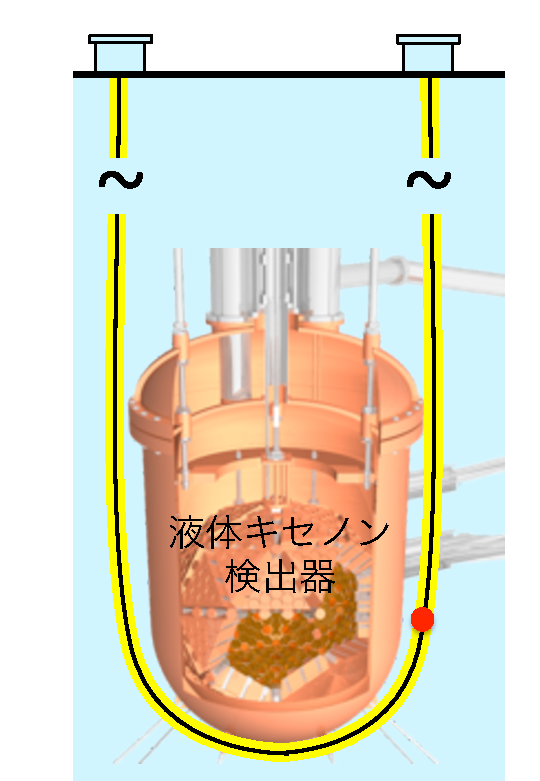
\includegraphics[width=4.5cm]{detector.pdf}
		         \caption{XMASS検出器と外部較正装置。中央の球形のものが液体キセノンのXMASS検出器本体で、銅製の真空容器の中に入っており、水色で示したように水タンク中に設置してある。改良前の外部較正装置は黄色で示したガイドチューブにワイヤーを通し線源を移動させていた。}
		         \label{fig:detector}
	         \end{center}
         \end{wrapfigure}

\textcircled{}研究の背景:暗黒物質とXMASS実験\par

申請者はこれまで2年間、XMASS実験に参加し暗黒物質探索を行ってきた。暗黒物質は全宇宙のエネルギーの約27\%を占めていると考えられており、原子からできている通常の物質の5倍も多く存在しているにも関わらず、重力相互作用をするという以外にその性質が分かっていない。これを明らかにすることは宇宙物理学や素粒子物理学において非常に重要な課題である。暗黒物質の正体については様々な候補があるが、Weakly Interacting Massive Particles (WIMPs)と呼ばれる素粒子であるという考えが有力である。XMASS実験はこのWIMPsを直接検出し{\bf \textcolor{red}{\ulinej{世界で初めて暗黒物質を発見する}}}ことを目的としている。XMASS検出器は835 kgの液体キセノンを使用した世界最大の暗黒物質検出器である(図\ref{fig:detector})。\par
暗黒物質の信号は、暗黒物質と地球の相対速度の変化によって季節変動する。これを観測することは暗黒物質の強力な証拠となる。既に、DAMA/NaI実験とそれをアップグレードしたDAMA/LIBRA実験では、暗黒物質の季節変動を発見したと主張している\cite{DAMA}。しかしその結果から導かれる暗黒物質の質量と散乱断面積の存在領域は、LUX実験\cite{LUX}などの結果と矛盾している。ただしLUXなどは探索手法に季節変動を用いておらず、DAMA実験の結果を完全に反証するには至っていない。DAMAではNaI検出器を14年間運転した1.33トン・年分のデータがあり、これと同等の統計量を得るには同等かそれ以上の質量の検出器を用いるしかない。835 kgの液体キセノンを用いた{\bf \textcolor{red}{\ulinej{XMASS検出器は1年でDAMAと同等の統計量を得られるため、この問題に決着をつけるのに最適な検出器である}}}。申請者はこの特長を活かし、{\bf \textcolor{red}{\ulinej{申請者の考案した外部較正装置によって系統誤差を最大限に小さく抑えて暗黒物質の季節変動探索を行う}}}。

\textcircled{}外部較正装置\par
検出器を運転するには、その検出器の特性を知るための較正が必ず必要になる。XMASSでは従来、液体キセノン中に線源を導入しデータ取得をすることによって検出器較正を行ってきた(内部較正)。しかしこの場合、検出器を開ける作業が伴うため、検出器の安定性を乱す。例えば、液体キセノンの入っている真空容器内の温度は約-100$^\circ$Cに保たれているが、内部較正を行うと0.01$^\circ$C上昇し、元の温度に戻るのに2日間を要する。また、較正時に光電子増倍管を1本外す必要があるため、暗黒物質測定時と完全に同じ状態で較正を行うことができない。これらの理由のため、申請者は{\bf \textcolor{red}{\ulinej{検出器外側に線源を設置する外部較正装置の改良を行うことで内部較正の回数を極力減らすための研究を行った}}}。\par
%\textcircled{}モンテカルロシミュレーション\par
%暗黒物質やその他の放射線に対して検出器がどのように応答するかを知るのには、モンテカルロシミュレーション(MC)という手法を用いる。Geant4を基に作成したXMASSのMCでは、液体キセノンの吸収長、散乱長などがパラメータとして含まれている。これは、これらの値を検出器中で測定することが難しいためである。したがって、これらのパラメータを較正データを用いて決定しなければならない。このパラメータのチューニングには、検出器外の線源由来の$\gamma$線が液体キセノンに入り込み、キセノン中心部に再構成される事象を用いる。これらの事象は稀にしか起こらないため、非常に多くの統計量が必要になるが、XMASSのMCは検出器の詳細な部分まで忠実に再現しているため、プロセスに時間がかかる。{\bf \textcolor{red}{\ulinej{申請者はMCの高速化に取り組み大統計のMCデータを作成した}}}。
%         \begin{wrapfigure}{r}{5cm}
%         		\begin{center}
%		         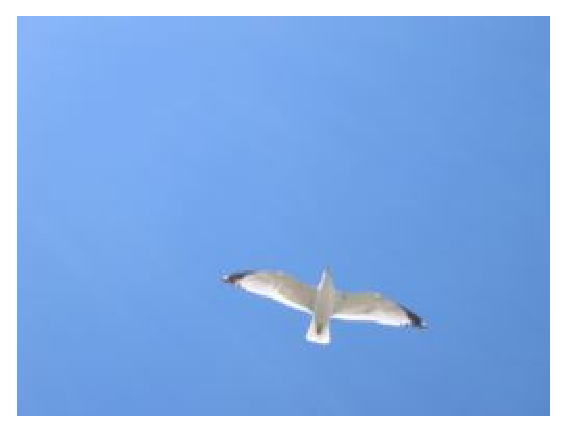
\includegraphics[width=5cm]{figs/seagull2.eps}
%		         \caption{カモメ}
%		         \label{fig:seagull}
%	         \end{center}
%         \end{wrapfigure}
{\bf 2. 申請者のこれまでの研究経過及び得られた結果}\par
\textcircled{}経過1. 外部較正装置の改良\par
上述のようにXMASS実験では液体キセノン中に線源を導入する内部較正を定期的に行っていたが、内部較正では検出器の安定性を損なうことが分かっていた。一方で、液体キセノンがどの程度$\gamma$線を遮蔽できるか(自己遮蔽能力)を調べるために外部較正も従来より行われていた。申請者は{\bf \textcolor{red}{\ulinej{外部較正が検出器の内部較正の主な目的である液体キセノンの発光量の測定に用いることが可能であると着想し、外部較正装置の刷新を行ってこの目的に用いることができるよう改良した}}}。改良前と改良後の外部較正装置を図\ref{fig:okahose}に示す。外部較正によって頻繁に発光量の測定を行うためには、手軽に操作が行えることと、測定の再現性を確保することが必要である。そのため、申請者は図中の細く描かれたチューブを導入した。線源はこの細いチューブの中をフィッシュテープと呼ばれる道具を用いて突き当たるまで送り出す。この仕組はBorexino実験\cite{Borexino}で採用されている較正装置を参考にした。
この方式によって毎回同じ場所で線源が固定され、{\bf \textcolor{red}{\ulinej{従来の装置では3\ cm程度であった線源の位置精度が5\ mm程度にまで改善された}}}。線源の導入についても、従来は必ず2人いなければできず複雑なため一部の共同研究者にしか扱えなかったが、手順を簡略化したことで、今後は毎週異なるシフト作業者が1人で較正作業を行うことができるようになり、
\begin{wrapfigure}{r}{3.8cm}
         		\begin{center}
		         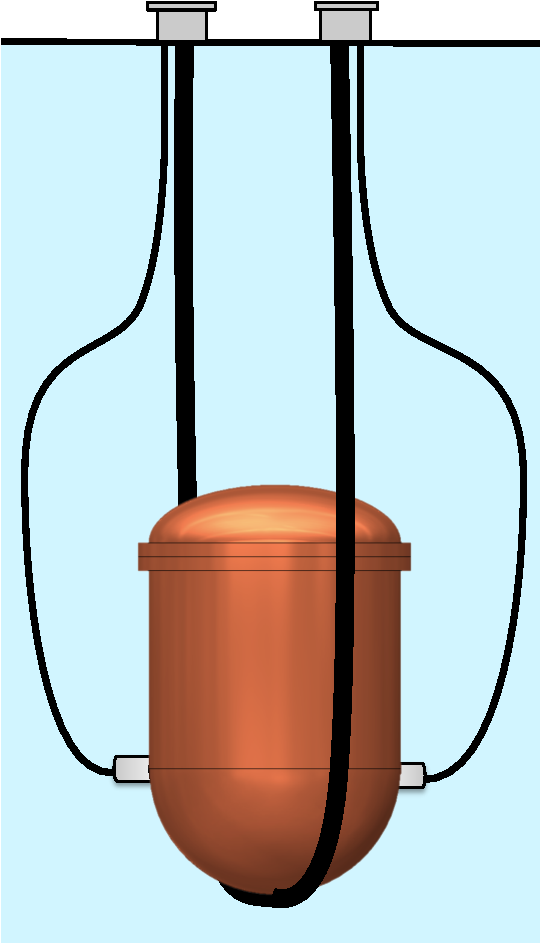
\includegraphics[width=4cm]{okahose.pdf}
		         \caption{改良した外部較正装置。新たに2本のチューブを導入し、従来のガイドチューブを遮光した。}
		         \label{fig:okahose}
	         \end{center}
         \end{wrapfigure}
これによって毎週欠かさず発光量を測定することができるようになった。この成果は日本物理学会において発表した(国内学会・シンポジウムにおける発表1, 2)。また、{\bf \color{red}{\ulinej{季節変動による暗黒物質の探索では数十 keV以下の低エネルギーの検出効率が重要であるため、この時間変化もモニターできるように今後改良を加える}}}。\par
\textcircled{}経過2. XMASS検出器の改造\par
2012年5月までのXMASSでの測定において予期せぬバックグラウンド事象(BG)が観測されたため、2012年の夏から2013年の秋にかけ、BG低減のため検出器の改造を行った。申請者は他の共同研究者と協力して検出器の改造作業を行った。改造の結果、観測データの5 keV以上の領域では予定通りBGが10分の1に削減された。5 keV以下の領域についても現在BGの理解が進んでいる。\par

\textcircled{}経過3. 外部較正データを用いたモンテカルロシミュレーションの改良と検出器由来$\gamma$線バックグラウンドの評価\par
%\textcircled{}外部$\gamma$線バックグラウンドの見積り\par
外部較正のデータを用いてモンテカルロシミュレーション(MC)の改良を行った。また、改良したMCを用いて検出器材料由来のバックグラウンド(BG)事象の影響を評価を行った(国内学会・シンポジウムにおける発表3, 4)。\\
%申請者は修士論文の研究として、検出器材料に含まれる放射性同位体(RI)からの$\gamma$線の影響を評価した。光電子増倍管(PMT)を固定するホルダー、真空容器、などの材料に含まれるRIの量は別の共同研究者によって測定されていたため、その値を用いて約100個の検出器材料中でRIが崩壊するモンテカルロシミュレーション(MC)を行い、測定に及ぼす影響を定量的に評価した。MCは申請者が外部較正のデータと比較することで、$\gamma$線の振る舞いを正確に予言するように改良した。MCの結果、調べた材料に含まれるRIの影響は既に別の共同研究者によって評価されていたPMT由来の$\gamma$線の影響に対して100 keVにおいて最大25\%と分かり、現在のXMASSのバックグラウンドレベルでは問題にならないことが分かった。この研究により、各場所で銅容器や液体キセノンの遮蔽がどの程度効くかが詳しく分かった。この結果はXMASSの次世代検出器のデザインにも役立てることができる。
 \par
\begin{thebibliography}{99}
\setlength{\itemsep}{-5pt}  % Adjust Item Separation
	\bibitem{DAMA}Bernabei, R. \textit{et al}., \textit{Eur. Phys. J. C} \textbf{73} (2013) 2648.
	\bibitem{LUX}Akerib, D.S. \textit{et al}.,  \textit{Phys. Rev. Lett.} \textbf{112} (2014) 091303.
	\bibitem{Borexino}Back, H., \textit{et al.},  arXiv:1207.2816 [physics.ins-det] (2012).
\end{thebibliography}


%end  現在までの研究状況 ====================
}

\newcommand{\研究の背景}{%
%begin  研究の背景===================
         \begin{wrapfigure}{r}{5cm}
         		\begin{center}
		         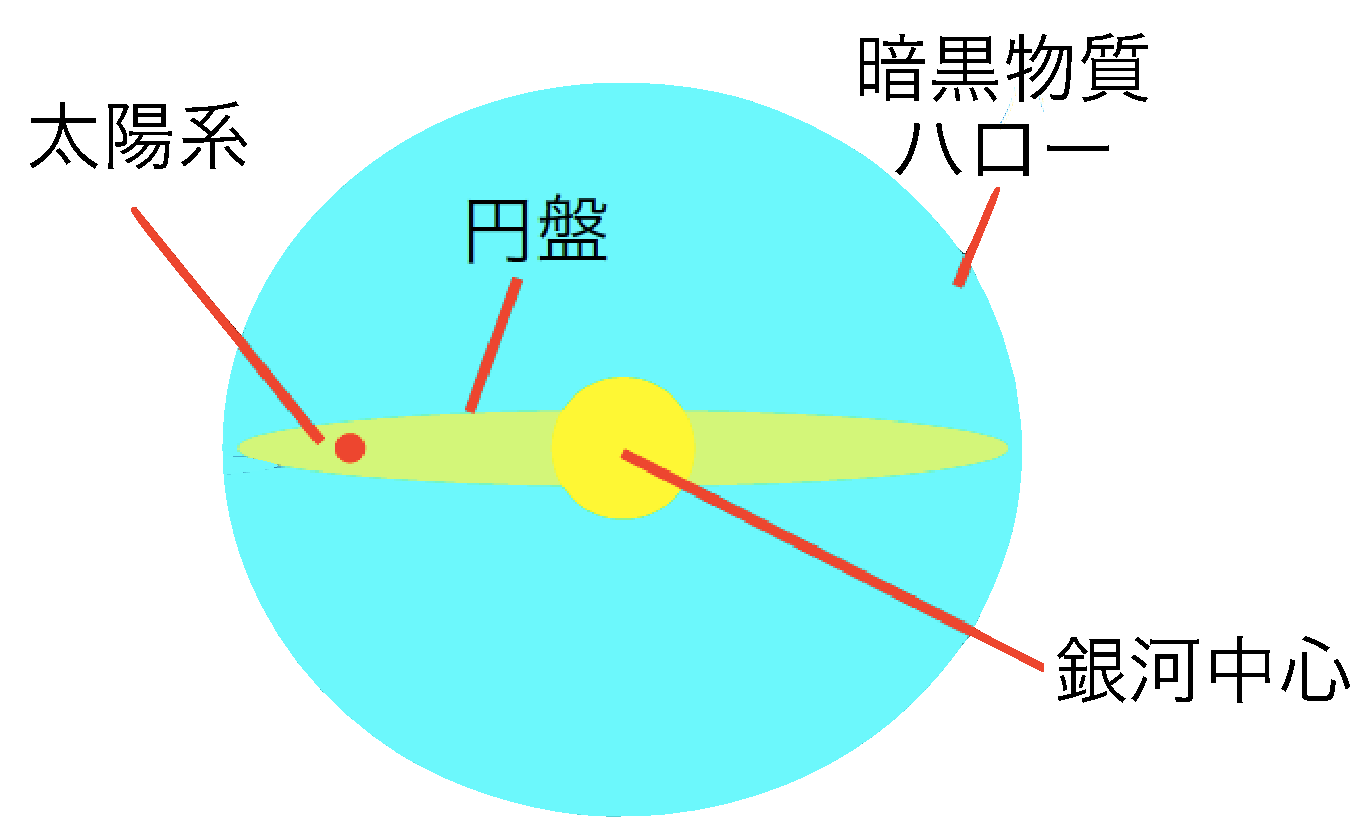
\includegraphics[width=5cm]{halo.pdf}
		         \caption{銀河中の暗黒物質の分布}
		         \label{fig:halo}
	         \end{center}
%         \end{wrapfigure}

\setcounter{figure}{4}
%         \begin{wrapfigure}{r}{5cm}
         		\begin{center}
		         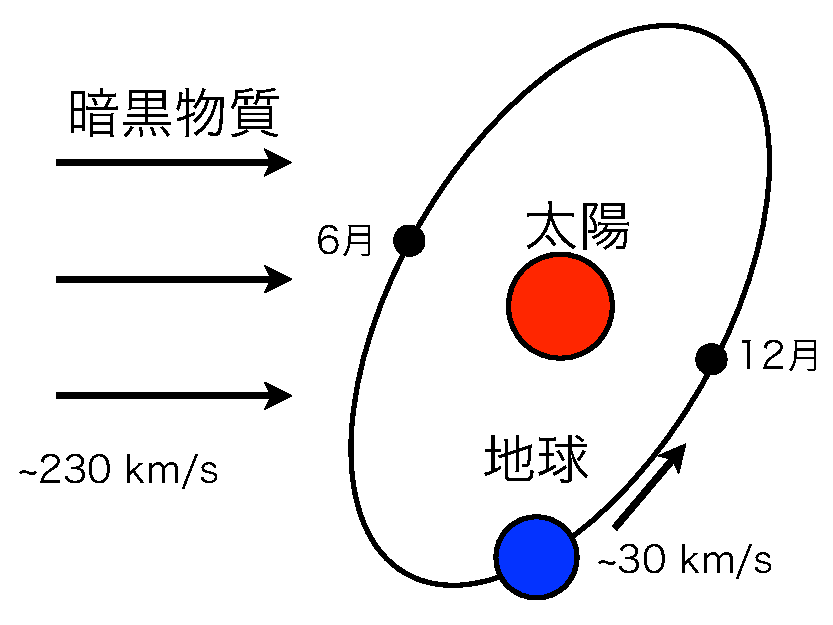
\includegraphics[width=5cm]{annual_modulation.pdf}
		         \caption{暗黒物質信号の季節変動}
		         \label{fig:annual}
	         \end{center}
         \end{wrapfigure}
暗黒物質は銀河系を覆うハロー状に存在していると考えられる。暗黒物質の平均速度は銀河に対して静止していると考えられるので、太陽系は暗黒物質の「風」を受けながら銀河系を約230 km/sで移動している。地球が太陽の周りを約30 km/sで公転していることにより、地球の銀河系に対する相対速度が最大になる6月は、地球と暗黒物質の衝突が最も多くなり、逆に12月は最も少なくなる。このため、検出器で検出される暗黒物質の信号レートも6月が最大、12月が最小となるはずである。もし信号がこのような周期を持てば、それが暗黒物質由来であることの強力な証拠となる。しかしこの{\bf \textcolor{red}{\ulinej{季節変動を観測するためには、信号レートの変化を精度よく測定することが必要であり、そのためには事象の検出効率が時期ごとに正確に分かっていなければならない}}}。そこで申請者は検出効率のモニタリングに外部較正のデータを用いることを着想した。%\par
%また、夏と冬でのエネルギースペクトルの形状の違いを世界で初めて観測できる可能性がある。

%XMASS検出器ではこれらの実験よりもよい感度で観測を行うことができる。
\def\damasize{11cm}
%\def\damasize{2cm}


%         \begin{wrapfigure}{l}{\damasize}
%        \begin{figure}
%
		         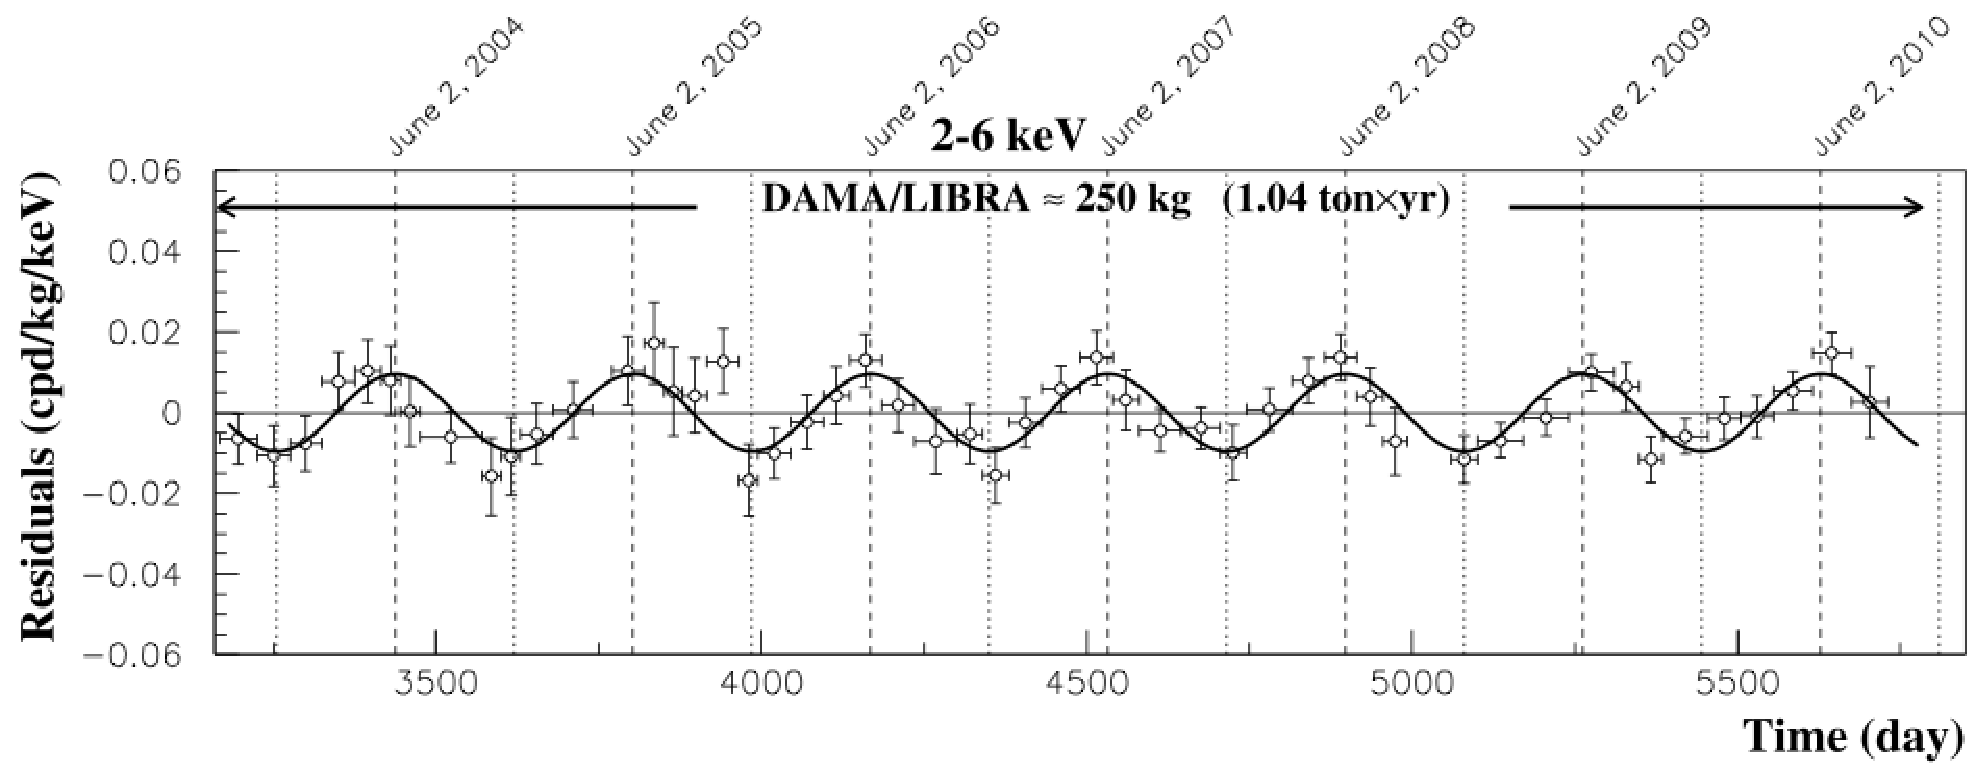
\includegraphics[width=\damasize]{dama.pdf}
%		         \caption{暗黒物質の季節変動}
         		\begin{center}
図4: DAMA実験による事象数の季節変動の結果 (Bernabei, R. \textit{et al}., (2013))
%		         \label{fig:dama}
%        \end{figure}
	         \end{center}
%         \end{wrapfigure}


%turn over (cross point)が見える。


%	\begin{thebibliography}{99}
%		\bibitem{teramuraKing} 寺村輝夫、「ぼくは王様 - ぞうのたまごのたまごやき」.
%	\end{thebibliography}
%end  研究の背景 ====================
}

%form: dc_form_05.tex ; user: dc_05_purpose.tex
%========== DC =========
%===== p. 05 研究の目的・内容 =============
\subsection{研究の目的・内容}
\newcommand{\研究目的}{%
%begin  研究目的と内容===================
\textcircled{}研究目的\par
         \begin{wrapfigure}{r}{7.8cm}
         		\begin{center}
		         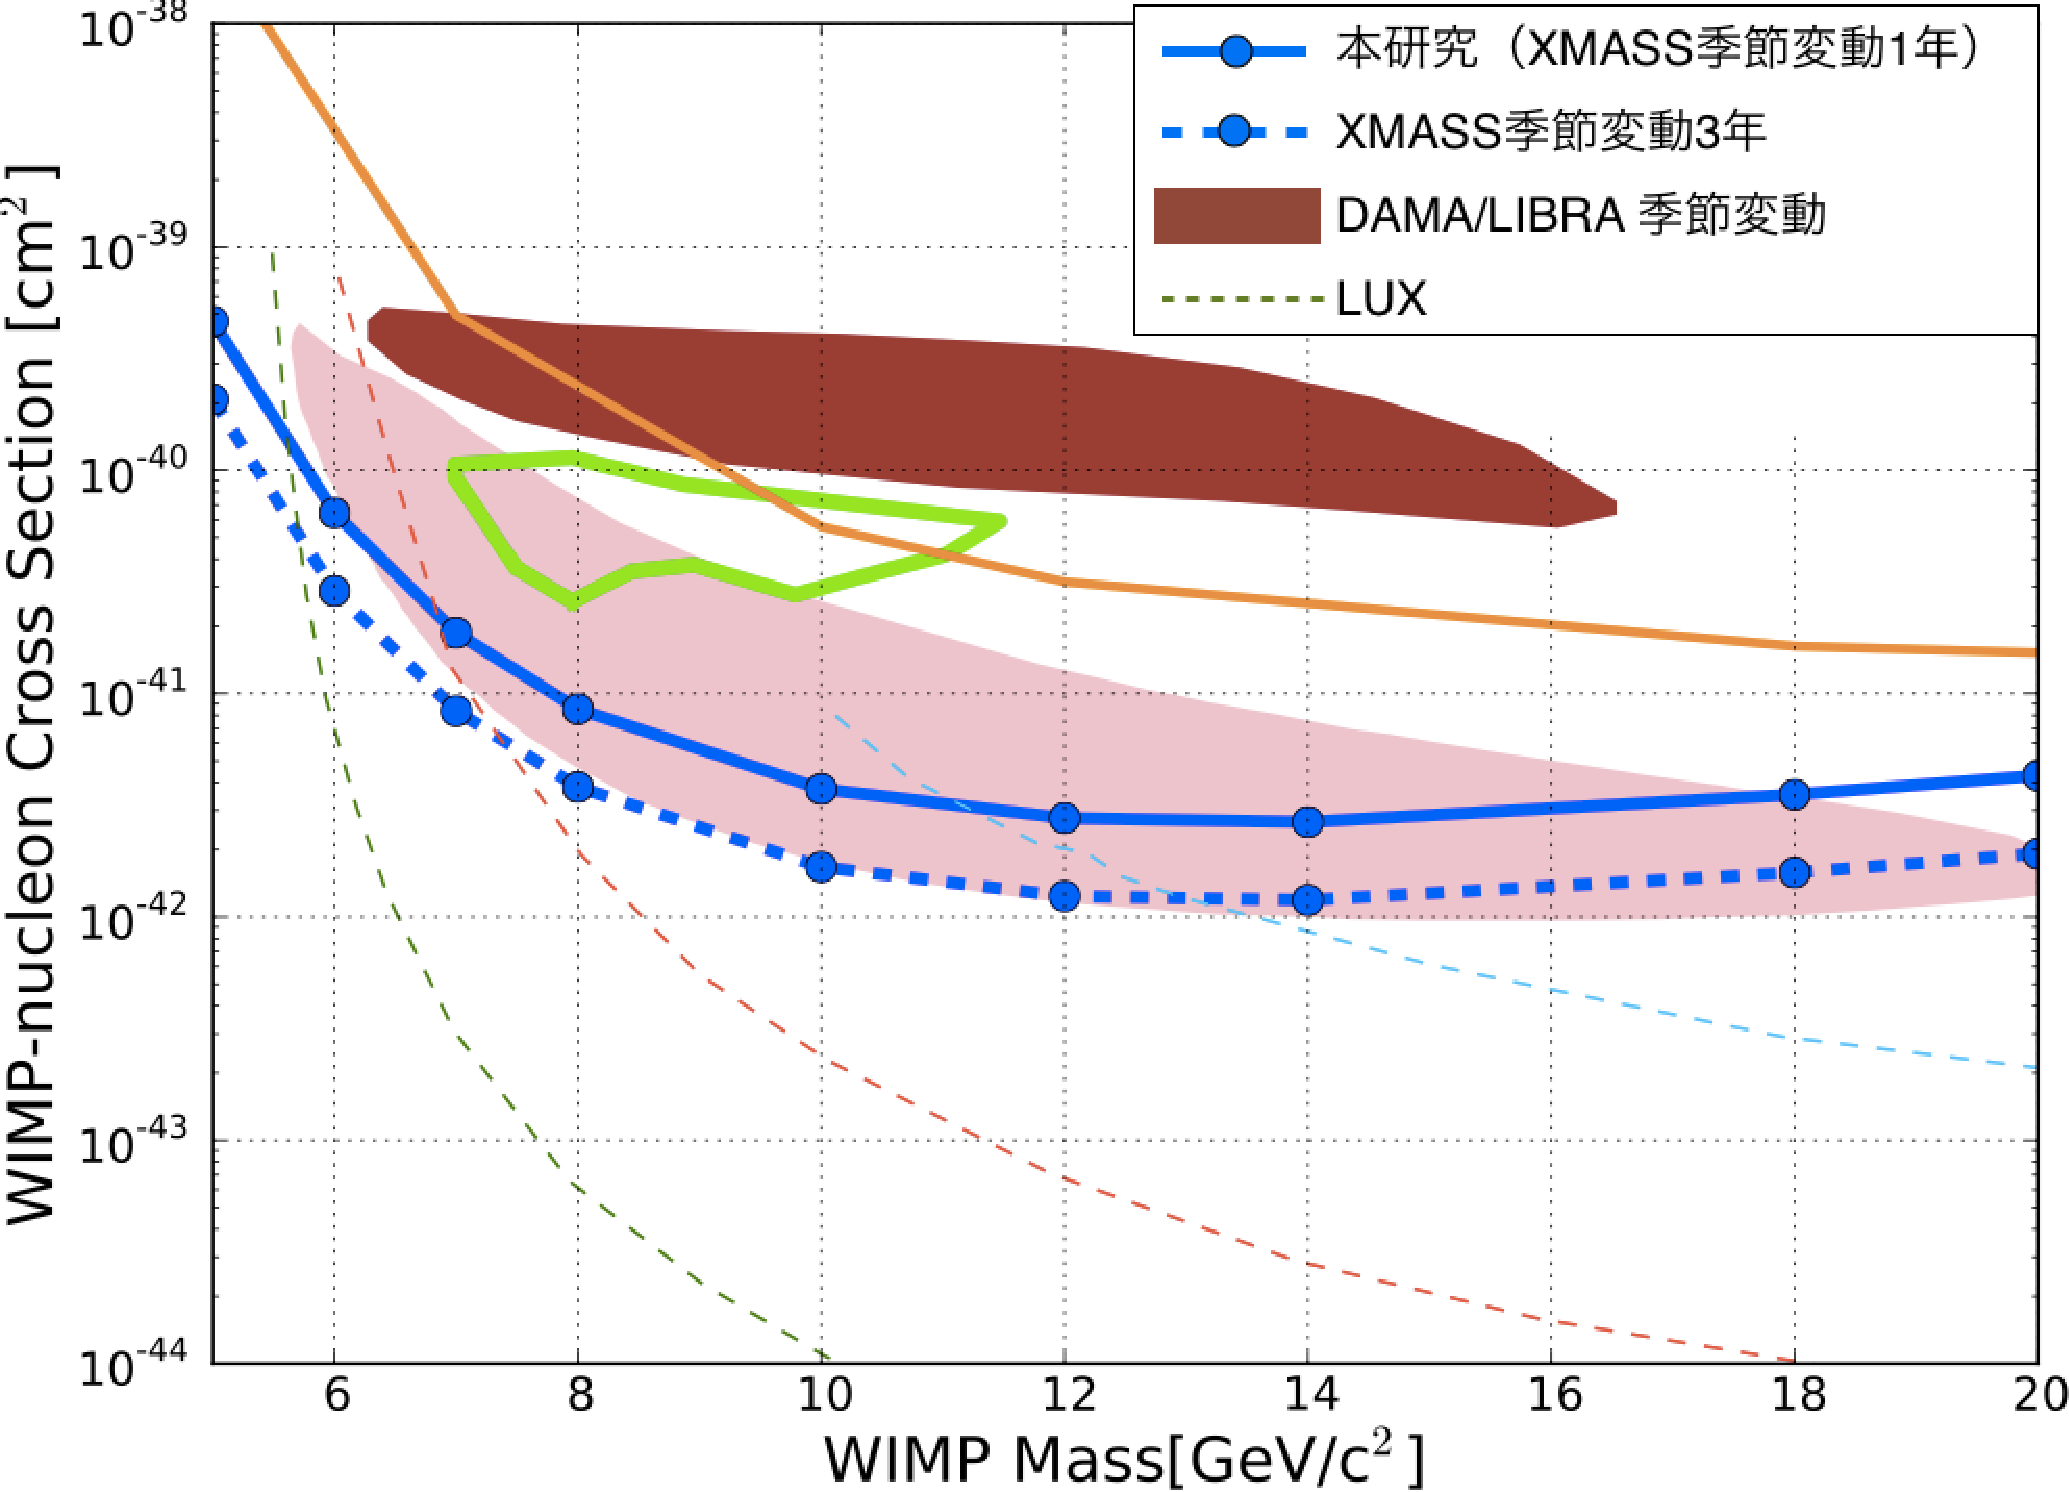
\includegraphics[width=8cm]{sensitivity.pdf}
		         \caption{改造後のXMASS検出器で期待される季節変動による暗黒物質探索の感度。}
		         \label{fig:sensitivity}
	         \end{center}
         \end{wrapfigure}
本研究ではXMASS検出器を用いて{\bf \color{red}{\ulinej{世界最高感度で季節変動による暗黒物質探索を行う}}}。右の図\ref{fig:sensitivity}に改造後のXMASS検出器で期待される季節変動による暗黒物質探索の感度を示す。横軸は暗黒物質の質量、縦軸は暗黒物質と核子の散乱断面積を示す。濃い赤がDAMA/LIBRA、薄いピンクがCDMS(Si)、緑がCoGeNTによってそれぞれ存在が主張されている領域で、このうちDAMA/LIBRAのみが季節変動を用いた結果である。曲線はそれより上の領域での暗黒物質の存在を排除したことを示し、オレンジが改造前のXMASS、水色の点線がCDMS、赤い点線がXENON100、緑の点線がLUX実験によるものであり、いずれの結果も季節変動による方法を用いていない。改造後のXMASSにおいてエネルギー閾値0.3 keVで季節変動による測定を行った場合に期待される感度を青い実線(1年間の観測)、点線(3年間の観測)で示す。測定の結果、暗黒物質の存在が確認できなかった場合これらの線より上の領域が排除されることになる。これを実現するために、以下のようなトピックごとに研究を進める。
\par
\textcircled{}外部較正による検出器のモニタリング\par
共同研究者と協力し、申請者が導入した外部較正装置を用いて毎週データを取得する。申請者はそのデータを利用して{\bf \color{red}{\ulinej{液体キセノンの発光量と低エネルギー事象の検出効率をそれぞれ0.5\%と1\%の精度でモニターする}}}。\par
%\textcircled{}季節変動を用いた暗黒物質探索\par
$\largestar$ データ取得システム(DAQ)の改良\par
現在のXMASS検出器では、データ取得は最大約100 Hzで行うことができ、これに適した強度の$^{60}$Co線源を用いて外部較正を行っている。データ取得を律速しているのはフラッシュADC(FADC)のデータ転送である。申請者はFADCデータ保存ディスクを分散化したシステムの構築しデータ転送の効率化を行うことで、データ取得を最大1 kHzで行えるよう改良する。これによって{\bf \color{red}{\ulinej{現在の10倍の強度の線源を用いて短い時間で大量の事象を得ることができるようになる}}}。\par
$\largestar$ 外部較正線源の位置再現性の改良\par
申請者が導入した現在の外部較正装置では、ガイドチューブの終端での詳細の線源の位置を知ることができないため、線源の位置再現性は最大5 mmとしている。DAQの改良によって1 kHzでデータ取得を行うことができれば、現在よりも大強度の線源を用いて較正を行うことができる。これにより$^{60}$Coでの1時間の測定で360万事象が得られ、0.05\%で位置の不定性を調べることができる。これは{\bf \color{red}{\ulinej{0.2\ mmの不定性に対応する}}}。
%これを1 mmまで改良する。これによって、レートの不定性は1.5\%から1.0\%に向上する。
\par
$\largestar$ 外部較正による低エネルギーの事象検出効率のモニタリング\par
季節変動を用いて暗黒物質探索を行うには、月ごとの事象数の変化を見る必要があるため、暗黒物質の信号領域である低エネルギー事象(0.3 keVから数keV)に対しての検出効率を各時期ごとに把握しておく必要がある。上述のDAQと位置再現性の改良によって、毎週の外部較正によって液体キセノンの発光量のモニタリングとともに、低エネルギー事象検出効率のモニタリングも1\%の精度で行えるようになる。

\textcircled{}低エネルギーBGの理解と変動の評価\par
経過3で述べたような申請者のこれまでのMCの経験を活かし、外部較正データの1 MeV程度の高エネルギー事象をコントロールサンプルとして用いてMCの改良を行う。{\bf \color{red}{\ulinej{改良したMCを低エネルギーBGの理解に用いて、短寿命核種由来などによるBG変動が暗黒物質の季節変動の測定に与える影響を評価する}}}。\par

\textcircled{}季節変動を用いた暗黒物質探索\par
\par
申請者は2015年度の最初の半年で上記予備研究を完了し、その後の1年半の間に暗黒物質観測データとともに外部較正データを毎週取得し、季節変動の解析を行う。

%\vskip{5cm}
%検出器への影響を最小限にし、暗黒物質の測定時間を減らさないよう、超新星爆発、シフトの負担を減らす
%などの目的のために、データは短い時間で取得することが望ましい。


%	トリガーの開発

	
%	DAQのアップグレード
	

	
%	BG レベル
	
%	DAMAはNaIいっぱいなのでsystematic errorが??
	
%end  研究目的と内容 ====================
}

%form: dc_form_06.tex ; user: dc_06_plan.tex
%========== DC =========
%===== p. 06 研究の特色・独創的な点、年次計画 =============
\newcommand{\研究の特色と独創的な点}{%
%begin  研究の特色と独創的な点===================
{\bf \textcircled{} 先行研究と比した本研究の特色、着眼点、独創的な点}\par
既に述べたようにXMASS検出器は現時点で{\bf \color{red}{\ulinej{世界最大の暗黒物質検出器であり、期待される暗黒物質事象も最も多い}}}。この特長は暗黒物質の季節変動の探索において極めて有利である。もうひとつの大きな特長として、XMASS検出器は液体キセノンの高い発光量のために、0.3 keVという極めて低い閾値を実現している(DAMA実験は2 keV)。{\bf \color{red}{\ulinej{暗黒物質による事象数はエネルギーが低くなるほど指数関数的に増大するので閾値が低いことも有利に働く}}}。
また、XMASS検出器はシンチレーション光のみを用いている(一相式と呼ばれる)ため、同じく液体キセノンを用いているLUX実験などの電子のドリフトを利用する検出器(二相式と呼ばれる)ではできない高いレートでのデータ取得が行える。本研究では高レートでの外部較正により、{\bf \color{red}{\ulinej{検出器への影響を最小限に抑えながらも、稀にしか起こらない10\ keV以下の低エネルギー事象をモニターすることができる}}}。さらに、DAMA実験では暗黒物質がすると考える原子核反跳事象と、ガンマ線などによる電子事象のどちらも測定し、モデルに依存しない測定を行っているが、二相式の検出器ではこれに対して充分な感度を出せない。XMASSでは充分な発光量を持ち低BGであるため高感度でモデルに依存しない測定を行うことができる。
\par
{\bf \textcircled{} 本研究の位置付け、意義と完成したとき予想されるインパクト及び将来の見通し}\par
本研究では、DAMA/NaI実験によって1997年に最初に報告され、20年近く決着がついていない現象について、DAMAと同等の統計量によって決着をつける。これは、現時点で世界最高感度を達成しているLUX実験や、{\bf \color{red}{\ulinej{他のどの検出器にもできないことである}}}。探索の結果DAMA実験と同様の結果を得て新現象の発見となった場合、もしくはDAMAとは矛盾した結果が出た場合のどちらであっても今後の暗黒物質直接探索において重大な影響を与える。本研究の完成後は大型化した次世代検出器(XMASS-1.5)での測定を開始し、さらに詳細な研究を行う。

%系統誤差
%end  研究の特色と独創的な点 ====================
}


\newcommand{\年次計画1年目}{%
%begin  年次計画1年目===================
\textcircled{}外部較正手法の確立\par
最初の半年間で外部較正によって液体キセノンの発光量と低エネルギーの検出効率をモニターする方法を確立する。まず、データ書き込みディスクの分散化によってFADCのDAQの高速化を行う。DAQの高速化が実現すれば、強い線源を用いることにより位置再現性の高い外部較正が行えるようになり、低エネルギーの検出効率をモニターできるようになる。\par
\textcircled{}外部較正データの取得\par
次の半年間で、この新しい方法による外部較正データの取得を開始する。較正データの取得は共同研究者と協力し毎週行う。同時に較正データの解析を開始し、液体キセノンの発光量、低エネルギー事象の検出効率の時間変化を調べ、季節変動の測定への影響を評価する。\par
\textcircled{}MCの改良\par
また、外部較正データをコントロールサンプルとして用いて、液体キセノンの吸収長、散乱長などの値を調べ、データを正確に再現するMCを作成する。また、暗黒物質探索のデータ取得も共同で行う。

%	\vspace{2cm}% adjust the length if necessary
%end  年次計画1年目 ====================
}

\newcommand{\年次計画2年目}{%
%begin  年次計画2年目===================
\textcircled{}暗黒物質探索データの解析\par
引き続き暗黒物質探索のデータ、外部較正データの取得を継続する。これによって得られた1.5年分の探索データを用いて季節変動による暗黒物質探索の解析を行い、結果を論文にまとめて投稿する。この際、外部較正のデータから得られた発光量、低エネルギー事象の検出効率の時間変化と、作成したMCを系統誤差を評価するのに用いる。また、MCによって暗黒物質と検出器の反応を予測し、得られた実験結果とを比較することで、データを暗黒物質として解釈できるかなどを共同研究者と議論する。

%	\vspace{4cm}% adjust the length if necessary


%end  年次計画2年目 ====================
}

\newcommand{\年次計画3年目}{%
%begin  年次計画3年目===================
%	\vspace{3cm}% adjust the length if necessary
%end  年次計画3年目 ====================
}

%form: dc_form_07.tex ; user: dc_07_rights.tex
%========== DC =========
%===== p. 07 人権の保護及び法令等の遵守への対応 =============
\subsection{人権の保護及び法令等の遵守への対応}
\newcommand{\人権の保護及び法令等の遵守への対応}{%
%begin  人権の保護及び法令等の遵守への対応 ===================
該当しない。
%end  人権の保護及び法令等の遵守への対応 ====================
}

%form: dc_form_08.tex ; user: dc_08_publications.tex
%========== DC =========
%===== p. 08 研究業績 =============
\section{研究業績}
\subsection{学術雑誌(紀要・論文集等も含む)に発表した論文及び著書}
\newcommand{\学術雑誌等に発表した論文または著書}{%
%begin  学術雑誌等に発表した論文または著書===================	
	\begin{enumerate}
		\item[](査読有り)%===========================
		\item K. Abe, K. Hieda, K. Hiraide, S. Hirano, Y. Kishimoto, K. Kobayashi, S. Moriyama, K. Nakagawa, M. Nakahata, H. Ogawa, \ulinej{N. Oka} (11番目), H. Sekiya, A. Shinozaki, Y. Suzuki, A. Takeda, O. Takachio, K. Ueshima, D. Umemoto, $\cdots$, K. Miuchi, $\cdots$, S. Nakamura, (28名省略),
		``Light WIMP Search in XMASS'', 
		\textit{Physics Letters B}, Elsevier,  {\bf 719}, pp 78-82, (2013).

		\item K. Abe, K. Hieda, K. Hiraide, S. Hirano, Y. Kishimoto, K. Kobayashi, S. Moriyama, K. Nakagawa, M. Nakahata, H. Ogawa, \ulinej{N. Oka} (11番目), H. Sekiya, A. Shinozaki, Y. Suzuki, A. Takeda, O. Takachio, K. Ueshima, D. Umemoto, $\cdots$, K. Miuchi, $\cdots$, S. Nakamura, (28名省略),
		``XMASS Detector'', 
		\textit{Nuclear Instruments and Methods in Physics Research Section A}, Elsevier,  {\bf 716}, pp 78-85, (2013).

		\item K. Abe, K. Hieda, K. Hiraide, S. Hirano, Y. Kishimoto, K. Kobayashi, S. Moriyama, K. Nakagawa, M. Nakahata, H. Ogawa, \ulinej{N. Oka} (11番目), H. Sekiya, A. Shinozaki, Y. Suzuki, A. Takeda, O. Takachio, K. Ueshima, D. Umemoto, $\cdots$, K. Miuchi, $\cdots$, S. Nakamura, (28名省略),
		``Search for solar axions in XMASS, a large liquid-xenon detector'', 
		\textit{Physics Letters B}, Elsevier,  {\bf 724}, pp 46-50, (2013).

		\item[](査読なし)%=============================
		\item \ulinej{N. Oka}, S. Takakura, H. Kakubata, S. Umehara, K. Matsuoka, T. Kishimoto, A. Sakaguchi, M. Nomachi, and Y. Sugaya,  
				``Tomographic Measurement with Cosmic-ray Muons by using Large Plastic Scintillators'', 
				OULNS Annual Report 2010, Laboratory of Nuclear Studies, Osaka University, pp16-17, (2011).
	\end{enumerate}
%	注:著者の所属・職(論文発表時)\\
%	1: 大阪大学理学部学生、
%	2: 明治大学文学部学生、
%	3: 東京帝国大学医学部学生、
%	4: ミッキー大学教授、
%	5: Univ. of Zoo大学院生
%end  学術雑誌等に発表した論文または著書 ====================
}

\subsection{学術雑誌等又は商業誌における解説・総説}
\newcommand{\学術雑誌等または商業誌における解説や総説}{ なし%
%begin  学術雑誌等または商業誌における解説や総説===================
%	\begin{enumerate}
%\item[] なし
%	\end{enumerate}
%end  学術雑誌等または商業誌における解説や総説 ====================
}

\subsection{国際会議における発表}
\newcommand{\国際会議における発表}{ なし%
%begin  国際会議における発表===================
%	\begin{enumerate}
%\item[] 
%	\end{enumerate}
%end  国際会議における発表 ====================
}

\subsection{国内学会・シンポジウムにおける発表}
\newcommand{\国内学会やシンポジウムにおける発表}{%
%begin  国内学会やシンポジウムにおける発表===================
	\begin{enumerate}
      		\item[] (日本語口頭発表・査読なし)
		\item \textcircled{}\ulinej{岡直哉} 他XMASS Collaboration、「XMASS実験:外部較正装置の改良」 日本物理学会 2013年秋季大会、高知大学、2013年9月20日
		\item \textcircled{}\ulinej{岡直哉} 他XMASS Collaboration、「XMASS実験:外部ガンマ線源によるXMASS検出器の較正」日本物理学会 第69回年次大会、東海大学、2014年3月30日
		\item[]他1件 %(ICRR発表会)
      		\item[] (日本語ポスター発表・査読なし)
		\item \textcircled{}\ulinej{岡直哉} 「XMASS実験における検出器部材からのバックグラウンド事象の研究」原子核素粒子若手三者夏の学校、ホテルたつき、2013年8月5日
		\item[]他1件 %(ICRR発表会)
      		\item[] (英語口頭発表・査読なし)
		\item \textcircled{}\ulinej{N. Oka}, ``Study of BG Contribution from Outer Components'', XMASS Collaboration Meeting, Kamioka Observatory, 2012年9月30日
		\item[]他9件
	\end{enumerate}
%end  国内学会やシンポジウムにおける発表 ====================
}

\subsection{特許等}
\newcommand{\特許等}{ なし%
%begin  特許等===================
%	\begin{enumerate}
%\item[] なし
%	\end{enumerate}
%end  特許等 ====================
}

\subsection{その他の業績}
\newcommand{\その他の業績}{ なし%
%begin  その他の業績===================
%	\begin{enumerate}
%\item[] なし
%	\end{enumerate}
%end  その他の業績 ====================
}
%{\bf (5)特許等、(6)その他}
%	\begin{enumerate}
%\item[] なし
%	\end{enumerate}

\subsection{発表前}
\newcommand{\発表前の業績}{%
%begin  発表前の業績===================
%end  発表前の業績 ====================
}


%form: dc_form_09.tex ; user: dc_09_myself.tex
%========== DC =========
%===== p. 09 自己評価 =============
\section{自己評価}
\newcommand{\自己評価}{%
%begin  自己評価===================
{\bf 1. 研究職を志望する動機}\par
申請者は中学生の頃より、この宇宙がどのようにでき、存在しているかを知ることを熱望していた。高校に入り、この問題に物理学によってアプローチできることを知り、大学では物理を学ぶことを決めた。大学に入って物理学を学び、物理や自然科学がどのようなものであるか理解していくうちに、{\bf \textcolor{red}{\ulinej{科学の特徴である実証的側面を強く持つ実験物理学に魅力を感じた}}}。またそれ以前から、{\bf \textcolor{red}{\ulinej{世界で誰も見たことのない現象、事実を発見したい}}}という思いを強く持っていた。この2つの動機から研究職を志望している。\par
{\bf 目指す研究者像}\par
研究に没頭するとどうしても社会とのつながりが弱くなりがちである。しかし研究の喜びは自分で何かを発見することだけでなく、自分の知り得たことを他の人にも知ってもらうことにもあると思う。申請者は{\bf \textcolor{red}{\ulinej{自分の研究内容を積極的に社会へ発信していく研究者でありたい}}}。また最近、科学論文の改ざんが話題になった折、科学とはどういうものであるか市民にほとんど理解されていないということを感じた。科学者には自分の研究成果を世の中に伝えるだけではなく、科学とはなにかを伝える義務があると考える。このため、{\bf \textcolor{red}{\ulinej{科学の内容だけではなく、科学的なものの見方など、科学自体を知ってもらう取り組みをしたい}}}。\par
{\bf 自己の長所等}\par
{\bf \textcolor{red}{\ulinej{申請者の長所は研究を楽しむことができるということである}}}。目標とする成果を出すまでは失敗の連続であろうが、それすらも楽しめなければ研究を続けていくことはできない。また時として予想外の現象に悩まされることもあるが、なぜそうのようなことが起こるのかを考えること、また考えた結果、現象を理解できるという体験は研究や実験をしていく中で最も楽しいことである。\par
\vspace{5mm}
{\bf 2. 自己評価をする上で、特に重要と思われる事項}\par
\textcircled{}留学経験など\par
申請者は博士前期課程の2年間のほとんどを岐阜県飛騨市神岡町の茂住集落で過ごした。商店もなく最寄りのコンビニエンスストアまでは自動車で30分近くかかるというその環境に留学していたと言ってもよいと思う。スーパーカミオカンデ検出器をはじめ数々の実験施設のある神岡鉱山近くのこの集落には世界中から第一線の研究者や若い学生が集まり、彼らと交流しながら充実した研究生活を送ることが出来た。神岡で築いた交友関係以外にも、申請者はこれまで通った大阪大学、東京大学、神戸大学の各所においてよい友人、指導者に恵まれた。さらに2013年夏に行われた原子核三者若手夏の学校では、高エネルギーパートの幹事を務めた。夏の学校に参加したことで、多くの同じ道を志す仲間と知り合うことができた。{\bf \textcolor{red}{\ulinej{これらの人脈は、これから研究者として生活していく上で大切なものになると考えている}}}。\par
\textcircled{}研究能力\par
その神岡で申請者はXMASS実験に従事し、数々の貢献をした。年に数回、海外の共同研究者も集まって議論するコラボレーションミーティングでは2年間を通じて10度発表したことがその証拠と言える。この経験から、これからも実験を続けていくことに自信を持つことができ博士後期課程への進学を決意した。日々の研究活動においては、{\bf \color{red}{\ulinej{課された仕事をこなすだけではなく、自分で考えて工夫することを常に意識した}}}。2013年に行われたXMASS検出器の再建時に外部較正装置の再構築を担当することになった当初は、装置の小規模な改善を依頼されただけであったが、他の実験での較正装置を調査し、新方式の装置を同時に導入することによって外部較正に新たな役割を担わせることを着想した({\bf 2. 現在までの研究状況}を参照)。2日間に渡っての新装置の設置作業においては、責任者として現場の指揮にあたり、作業を無事に終了させた。この作業を通じて実験には段取りが非常に重要であることを学ぶことが出来た。また、XMASSグループでは毎週英語でミーティングを行っている。申請者はほぼ毎回発表し、発表能力、英語能力を日常的に磨いている。これらの能力は国際学会での発表や外国の研究者との議論するのに必須である。このように、研究を進めていく上で重要な能力を修士の間に身につけることができ、さらに高める努力を日々行っている。


%end  自己評価 ====================
}


%endUserFiles
% hook7 : right before including forms ============
 % for future maintenance

% dc_forms
%=======================================
\ifthenelse{\boolean{BudgetSummary}\OR\boolean{klTypesetPage0}}{
	%============================================================
%  Warning cover page
%============================================================

\begin{picture}(0,0)(\KLOddPictureX,\KLPictureY)
	\KLParbox{100}{700}{550}{600}{t}{
		\LARGE
		提出前に次の行を以下のようにコメントアウトし、\\
		コンパイルし直してください。\\
		\hspace{2cm}\%\textbackslash setboolean\{BudgetSummary\}\{true\}\\
		\hspace{2cm}\%\textbackslash KLTypesetPage\{..\}\\
		\hspace{2cm}\%\textbackslash KLTypesetPagesInRange\{..\}\{..\}\\
	}
	\西暦
	\KLParbox{100}{550}{500}{500}{t}{
		\begin{center}
			\LARGE 予算と研究組織のまとめ \\
			\Large \today
		\end{center}
	}

	\KLTextBox{100}{500}{550}{300}{}{
		\Large
		研究種目: \研究種目\研究種別\研究種目後半\\
		研究期間: \研究開始年度(H\研究開始元号年度) 〜 H\研究期間の最終元号年度\\
		研究課題名:「\研究課題名」\\
		研究代表者:\研究代表者氏名\\
		研究機関名:\研究機関名\\
	}
\end{picture}
\clearpage


}{}

\KLInputIfPageInRangeIsSelected{1}{2}{forms/dc_form_03-04}
\KLInputIfSelected{3}{forms/dc_form_05}
\KLInputIfSelected{4}{forms/dc_form_06}
\KLInputIfSelected{5}{forms/dc_form_07}
\KLInputIfSelected{6}{forms/dc_form_08}
\KLInputIfSelected{7}{forms/dc_form_09}
\KLInputIfSelected{8}{forms/dc_form_10}

%========================================


%endFormatFile

% hook9 : right before \end{document} ============
 % for future maintenance
\end{document}
